\section{Inclusión de librería a un proyecto: MATHLIB}


El proyecto sobre el cual se está trabajando utiliza en una de sus lineas la función \textit{cosf()} incluida desde la librería \textit{math.h}, sin embargo dado que es un proyecto pensado para ser implementado en una tarjeta LCDK que cuenta con un procesador de núcleo \textit{C674x}, es recomendable reemplazar dicha función por alguna provista por la librería \textit{MATHLIB}, que es recomendada por los fabricantes Texas Instrument (TI), en este caso se hará uso de la función \textit{cossp()}  (coseno \textit{single-precision}, para \textit{float} según MATHLIB).


Para esto se deben realizar algunos cambios en las configuraciones de compilación y enlace del proyecto. Primero se deben añadir las rutas que dirijan a los paquetes de la librería MATHLIB, como se muestran la figura \ref{path_mathlib}




\begin{figure}[H]
    \centering
    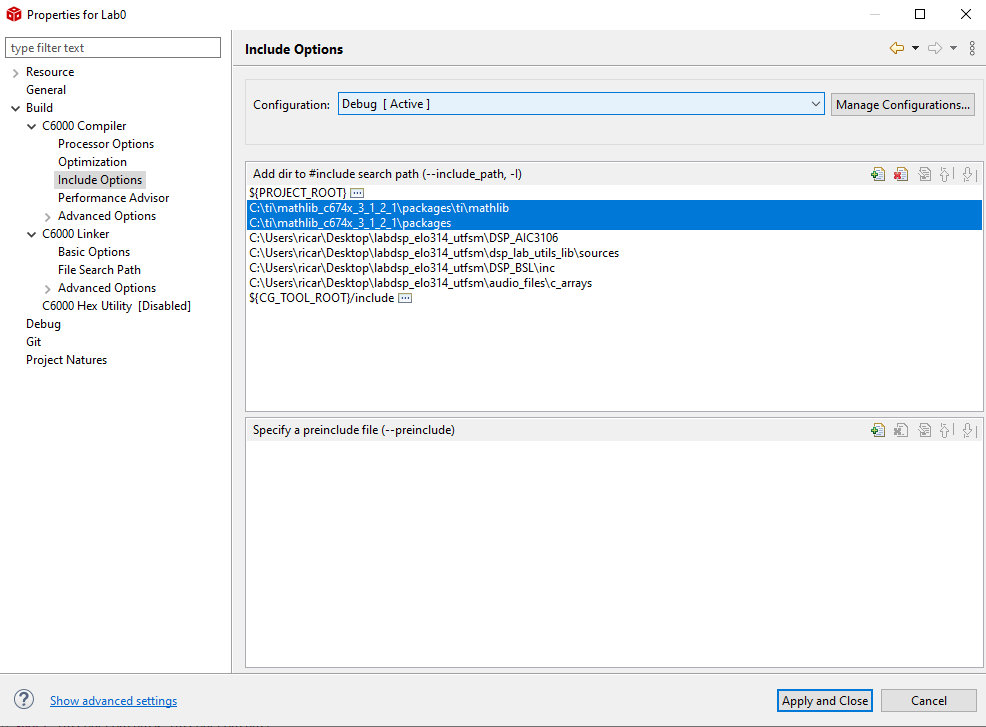
\includegraphics[scale = 0.6]{figures/mathlib_compiler.png}
    \caption{Configuración adicional al compilador para usar la librería MATHLIB}
    \label{path_mathlib}
\end{figure}


 Además se debe agregar la dependencia \textit{mathlib.lib}, indicando claramente el directorio en que se encuentra, esto se indica en la figura \ref{linker_mathlib}

\begin{figure}[H]
    \centering
    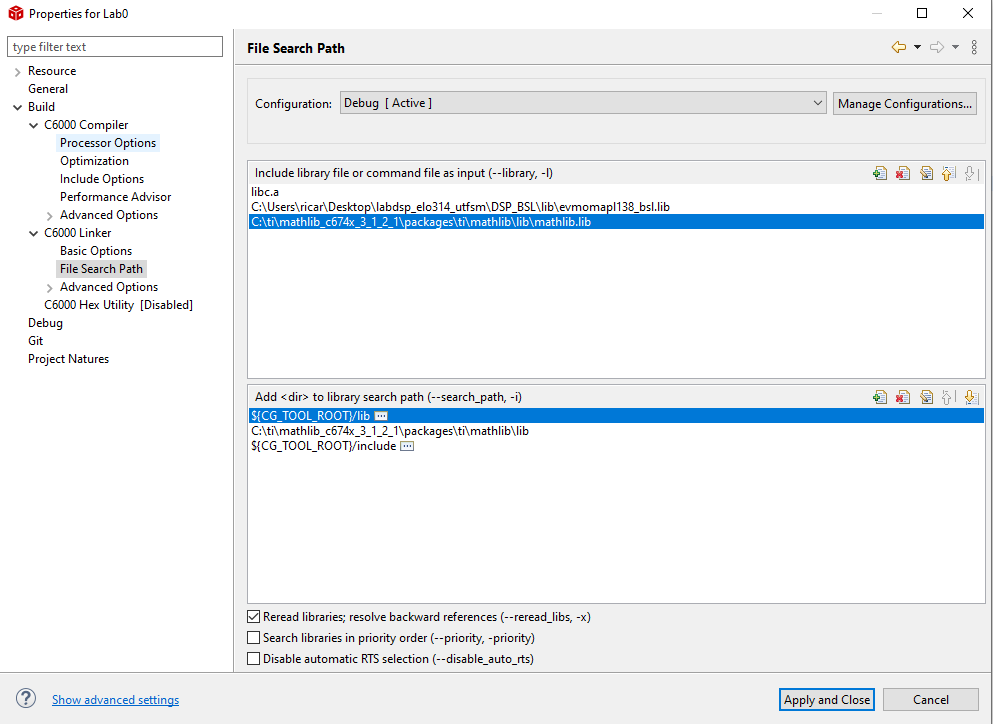
\includegraphics[scale = 0.6]{figures/mathlib_linker.png}
    \caption{Configuración adicional al \textit{linker} para usar la librería MATHLIB}
    \label{linker_mathlib}
\end{figure}

Además en la sección de inclusión de librerías del código en el archivo \textit{L1P2.c} se debe agregar la linea \texttt{\#include  ``mathlib.h''} y se debe modificar la línea 142 del código


\begin{lstlisting}[frame = single]
#include "mathlib.h"

...

...

%linea original
cosSignal = (int16_t)( 2 * ampCosine * cosf(thetaCosineSignal) );

%linea modificada
cosSignal = (int16_t)( 2 * ampCosine * cossp(thetaCosineSignal) );
\end{lstlisting}


Revisando la documentación asociada a la librería MATHLIB posee diversas funciones que permiten trabajar de forma sencilla con elementos matemáticos, entre ellas funciones trigonométricas, logaritmos, exponenciales, y potencias. Todas estas implementadas tanto para trabajar con datos de precisión simple y doble, permitiendo una versatilidad para diversas arquitecturas al trabajar con distinto número de bits.

Esto resulta beneficioso ya que al estar estas funciones ya implementadas en una librería se reduce considerablemente el tiempo de procesamiento al momento de ejecutar operaciones matemáticas al trabajar con enfoques en tiempo real.



